% =====================================================================
% DRAFT v0.1 -- IEEE JBHI submission
%
% STATUS: first draft. Every number in this file must be traceable to a
% table under outputs/tables/ produced by a script in this repository.
% Do not retype values. paper/check_numbers.py verifies the manuscript
% against those tables; run it before every commit.
%
% Items still open are marked \todo{} and listed in paper/OPEN_ITEMS.md.
% =====================================================================
\documentclass[journal]{IEEEtran}

\usepackage{booktabs}
\usepackage{graphicx}
\usepackage{amsmath}
\usepackage{url}
\usepackage[hidelinks]{hyperref}
\usepackage{xcolor}
\usepackage{siunitx}
\newcommand{\todo}[1]{\textcolor{red}{[TODO: #1]}}

\begin{document}

\title{How You Evaluate a Retinal Foundation Model Determines\\
       the Answer You Get}

\author{Shayan Abrar%
\thanks{Manuscript drafted \today. Code, experiment registry and all
generator scripts: \url{https://github.com/SHAYAN-ABRAR/Paper-Code}}}

\maketitle

% ---------------------------------------------------------------- abstract
\begin{abstract}
Domain-specific foundation models are increasingly the default starting point
for medical imaging, and linear probing is a common, computationally
inexpensive protocol for evaluating their representations. We ask whether that
protocol predicts what happens when the same models are adapted by
fine-tuning. We compare RETFound, a ViT-L/16 masked autoencoder whose
colour-fundus corpus is 904{,}170 photographs, against \emph{the exact ImageNet MAE checkpoint from
which it was initialised}. Architecture, objective, splits and schedule are held fixed, so the
intervention is the additional retinal-domain MAE continuation pretraining
itself. Under a frozen linear probe over
\num{10} seeds, the general-purpose initialisation transfers
better on two of three held-out domains ($+0.0626$ and
$+0.1134$ QWK, both $p<0.001$ after Holm correction). Under
identical partial fine-tuning of the last 4 of 24 transformer blocks, no
held-out domain shows a difference surviving correction. Testing the protocol
interaction directly on the \num{5} seeds common to both
protocols, the point estimates show substantial attenuation of the
ImageNet-MAE advantage on two domains with every seed agreeing in sign, but
the interaction does not reach multiplicity-adjusted significance at this seed
budget, and we do not claim the protocols are equivalent. In a
leave-one-domain-out evaluation on four public datasets, no
domain-generalization objective beat empirical risk minimisation, and three
separate effects were significant under a within-seed bootstrap at three
seeds and vanished at five. We argue that seed-level variance, not
test-set sampling variance, is the binding uncertainty in this problem.
\end{abstract}

\begin{IEEEkeywords}
Diabetic retinopathy, domain generalization, foundation models, model
evaluation, calibration, distribution shift.
\end{IEEEkeywords}

% ------------------------------------------------------------ introduction
\section{Introduction}
\IEEEPARstart{D}{iabetic} retinopathy screening is among the most successful
applications of deep learning in medicine, yet reported performance is almost
always measured on held-out images from the same source as the training data.
Deployment means something different: running on images from a clinic, camera
and population the model has never seen.

This paper reports a study of that gap on four public DR datasets treated as
distinct clinical domains, and arrives at a conclusion about \emph{measurement}
rather than about any particular method.

Our central observation concerns retinal foundation models. RETFound~\cite{zhou2023retfound}
is the reference self-supervised model for colour fundus photography and is
widely adopted as an initialisation. Its own checkpoint records that it was
initialised from a general-purpose ImageNet MAE ViT-L/16 and trained for a
further 801 masked-autoencoder epochs on retinal images. That makes an unusually
clean experiment available: compare RETFound against \emph{the checkpoint it was
built from}, with architecture, scale, objective, data splits, augmentation,
optimiser and schedule all held fixed. The model-level intervention is then the
additional retinal-domain MAE pretraining stage itself --- a training stage, not
merely a change of dataset.

Under a frozen linear probe, the general-purpose initialisation transfers
better on two of three held-out domains. Under identical \emph{partial}
fine-tuning (last 4 of 24 blocks) of both models, that advantage is no longer
statistically detectable on any domain. We test the protocol interaction
directly rather than inferring it from one comparison being significant and the
other not (Section~\ref{sec:interaction}). Linear probing is a common, computationally inexpensive way to evaluate a
foundation model's representation, while fine-tuning is how such models are
typically adapted in practice; the two protocols therefore support different
readings of the same comparison, although the interaction itself is not
established at this seed budget.

\textbf{Contributions.}
\begin{enumerate}
\item A matched-initialisation comparison of a domain-specific foundation model
      against its own general-purpose starting point, at two protocol levels
      (frozen probe and partial fine-tuning) on three held-out domains.
\item A direct test of the protocol interaction, rather than the common and
      invalid inference from one comparison being significant and another not.
\item A leave-one-domain-out evaluation of four domain-generalization
      objectives against ERM on two targets under two batch samplers, with
      diagnostics confirming each method's machinery engaged.
\item A quantification of what \emph{does} move cross-domain performance: a
      higher-resolution configuration exceeds every method and architecture
      change tested. A dedicated batch-size control separates resolution
      from the batch size confounded with it
      (Section~\ref{sec:resolution}).
\item A methodological result of independent interest: three effects in this
      study were significant under a paired bootstrap at three seeds and
      disappeared at five. We report all claims against an across-seed
      standard deviation as well as a bootstrap interval.
\end{enumerate}

% ----------------------------------------------------------- related work
\section{Related Work}

\textbf{Domain generalization.} A large family of objectives aims to learn
representations invariant to domain shift, including feature alignment
\cite{sun2016deepcoral}, style augmentation \cite{zhou2021mixstyle}, group
reweighting \cite{sagawa2020groupdro} and invariance penalties
\cite{arjovsky2019irm}. Gulrajani and Lopez-Paz \cite{gulrajani2021domainbed}
found that under a fair model-selection protocol none reliably outperforms
empirical risk minimisation on standard benchmarks. Our results reproduce that
conclusion on cross-domain DR grading and add an observation specific to
clinical data: these methods' machinery is frequently degenerate on naturally
imbalanced source pools, where a batch of 32 drawn from our pools contains zero
images from the smallest domain. We address this with a domain-balanced sampler
and an ERM control on that same sampler.

\textbf{Medical foundation models.} RETFound \cite{zhou2023retfound} applies
masked autoencoding \cite{he2022mae} to retinal images; the colour-fundus
checkpoint used here was pretrained on 904{,}170 photographs and is the
reference self-supervised initialisation for colour fundus photography.
Evaluations of such models commonly report linear-probe performance, since
probing is cheap and isolates representation quality from fine-tuning
hyperparameters. Our contribution is to run both protocols on a matched pair
--- the foundation model and the general-purpose checkpoint it was initialised
from --- and to show that they disagree.

\textbf{Evaluation under seed variance.} Reporting a single training run with a
test-set confidence interval remains common. We find that in this problem
seed-level variance exceeds test-set sampling variance often enough that three
separate effects were significant under a paired bootstrap and vanished when
two further seeds were added (Section~\ref{sec:seeds}).

% --------------------------------------------------------------- protocol
\section{Data and Protocol}

\subsection{Datasets}
Four public DR datasets are treated as distinct domains: DDR, APTOS~2019,
IDRiD and EyePACS, all graded on the five-point ICDR scale.
Table~\ref{tab:datasets} summarises them. \todo{insert
outputs/tables/table1\_dataset\_characteristics.tex}

\subsection{Leave-one-domain-out}
Each experiment trains on three domains and evaluates on the fourth, which
contributes \emph{test data only}. The held-out domain is excluded from
training, validation, early stopping, model selection and temperature fitting.
This is asserted in code rather than left to convention. Splits are
patient-level where patient identifiers exist.

\subsection{Statistical framework}
\label{sec:bars}
Two sources of uncertainty act on every comparison, and reporting either
alone is misleading here. Test-set sampling variance is what a conventional
paired bootstrap measures. Seed variance --- the fact that a different random
seed produces a different trained model --- is invisible to it, and in this
problem it is frequently the larger of the two.

\textbf{Uncertainty} is estimated with a crossed seed$\times$case
bootstrap. Because every seed is evaluated on the same test set, seeds and
cases are crossed rather than nested: each replicate resamples seeds with
replacement, draws \emph{one} case sample, and applies those same case indices
to every selected seed and to both models, preserving the pairing that gives
the design its power. Non-linear metrics are recomputed per seed and model on
the resampled cases rather than averaged from per-case values.

\textbf{Inference} is a paired test on the per-seed differences, with
Holm--Bonferroni correction across the pre-specified hypothesis family. This
is kept separate from the interval deliberately: an ordinary percentile
bootstrap resamples around the empirical distribution rather than under the
null, so its tail mass is not a calibrated $p$-value and is not reported as
one. An exact sign-flip permutation test is reported as a distribution-free
sensitivity check.

\textbf{Seed dispersion} --- the standard deviation of the paired per-seed
differences, and the number of seeds agreeing in sign --- is reported
throughout as a \emph{descriptive robustness diagnostic}. It is not a
significance criterion. An earlier version of this work used a
$|\Delta| >$ seed-SD threshold as an inferential rule; it has no
calibrated error rate and is retained only for description.

The need for the seed level is not hypothetical. Three separate effects in
this study cleared a within-seed paired bootstrap at three seeds --- two at
$p<0.001$ --- and disappeared when two further seeds were added
(Section~\ref{sec:seeds}, Fig.~\ref{fig:seeds}).

% ---------------------------------------------------------------- methods
\section{Methods}

\subsection{Matched foundation-model comparison}
RETFound's checkpoint metadata records
\texttt{resume=mae\_pretrain\_vit\_large\_full.pth}, mask ratio $0.85$, 801
epochs, \texttt{mae\_vit\_large\_patch16}. The named initialisation is
available publicly, so the control is not an approximation but the model
RETFound started from. Both are ViT-L/16 with $303.3$M parameters and identical
feature width.

\textbf{Frozen protocol.} Features are extracted once per backbone and
standardised per dimension using statistics fitted on the source training split
only. A linear head is trained for 200 epochs; the schedule was chosen by
convergence against an exact L-BFGS reference \emph{on source validation}, with
no target-test quantity involved in the choice.

\textbf{Partial fine-tuning protocol.} The last 4 of 24 transformer blocks are unfrozen,
which is $50.4$M of $303.3$M trainable and identical for both models. Both use
$\mathrm{lr}=10^{-4}$, batch 16, 20 epochs with early stopping.

\textbf{Leakage.} EyePACS is in RETFound's pretraining corpus and is therefore
excluded as a held-out target throughout; using it would report leakage as
generalization. This is enforced by a guard that raises rather than warns.
EyePACS remains a \emph{source} domain, which is sound, since source domains are
seen by construction. DDR, APTOS and IDRiD are not named in RETFound's
published colour-fundus pretraining corpus, whose composition is enumerated
in the source publication as 815{,}468 MEH-MIDAS and 88{,}702 EyePACS
photographs; we record them as \emph{not in the published corpus}. The
claim rests on that publication rather than on the checkpoint, which carries
no manifest of what it saw.

\subsection{Domain-generalization objectives}
Deep CORAL~\cite{sun2016deepcoral}, MixStyle~\cite{zhou2021mixstyle},
GroupDRO~\cite{sagawa2020groupdro} and IRMv1~\cite{arjovsky2019irm} are compared
against ERM at published defaults. Because a naturally shuffled batch from these
pools is dominated by one domain, each method is additionally run under a
domain-balanced sampler, \emph{with an ERM control on the same sampler}, and we
report how often each method's machinery was degenerate.

% ---------------------------------------------------------------- results
\section{Results}

\subsection{The two protocols disagree}
\label{sec:protocol}
Table~\ref{tab:foundation} and Fig.~\ref{fig:protocol} give the comparison.
Frozen, at ten seeds, the general-purpose initialisation is ahead on DDR
($+0.0626$) and APTOS ($+0.1134$), both established under
Section~\ref{sec:bars}. IDRiD points the other way ($-0.0429$, nine of ten
seeds agreeing) and its per-seed effect is significant after correction, but
its crossed interval spans zero on a 507-case test set; we therefore do not
claim it. Under partial fine-tuning, at five seeds, no target is established:
DDR $+0.0217$, APTOS $+0.0073$, IDRiD $-0.0423$. None survives correction, so
the correct statement is that no difference is demonstrated under this
protocol --- not that RETFound is favoured anywhere.

The mechanism is visible in the source--target split
(Fig.~\ref{fig:mechanism}). Frozen, both models fit
the source domains almost identically (within $0.017$ QWK on every target); the
entire difference is the drop from source to target, which is $5.9\times$ larger
for RETFound on DDR and $2.4\times$ larger on APTOS. Under partial fine-tuning, RETFound fits
the sources marginally better on all three targets. Whatever the frozen
representation lacked for transfer, four unfrozen blocks recover.

\begin{figure*}[t]
\centering
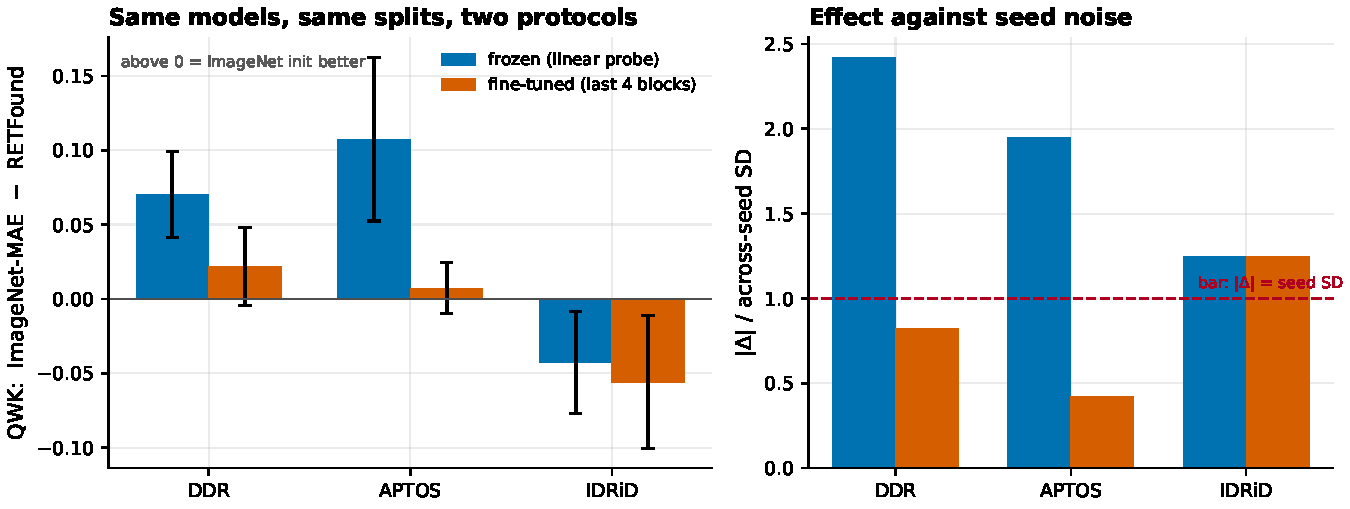
\includegraphics[width=\textwidth]{../outputs/figures/fig1_protocol_disagreement.pdf}
\caption{The same two models, same splits, two evaluation protocols. Left:
QWK difference (ImageNet-MAE minus RETFound) on each held-out domain; error
bars are the across-seed standard deviation of the paired per-seed differences.
Right: the same effects expressed as multiples of that standard deviation,
with the bar of Section~\ref{sec:bars} marked. The frozen protocol reports a
large advantage for the general-purpose initialisation on two domains; under
partial fine-tuning none is established, and the point estimate on the third
domain points the other way.}
\label{fig:protocol}
\end{figure*}

\begin{figure*}[t]
\centering
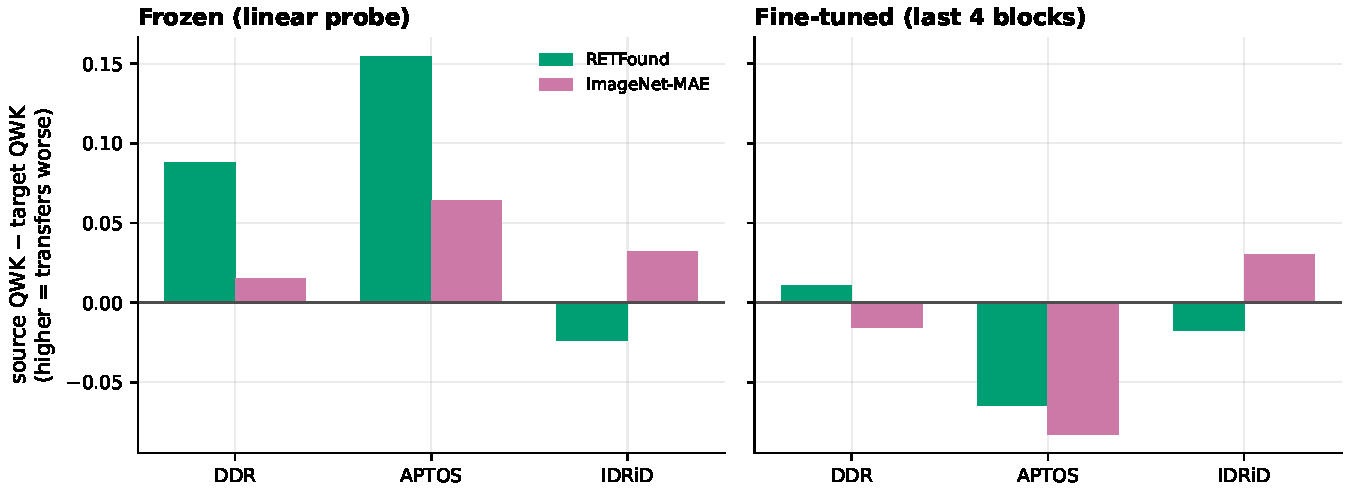
\includegraphics[width=\textwidth]{../outputs/figures/fig4_transfer_mechanism.pdf}
\caption{Why the frozen gap exists. Each bar is the drop from source-validation
QWK to held-out-target QWK, so a taller bar means the representation transfers
worse. Frozen (left), RETFound loses substantially more than the checkpoint it
was initialised from on DDR and APTOS despite fitting the source domains
equally well. Under partial fine-tuning (right), the difference closes.}
\label{fig:mechanism}
\end{figure*}

\subsection{Testing the protocol interaction directly}
\label{sec:interaction}
Observing that a difference is significant under one protocol and not under
another does not establish that the protocols differ; the two estimates can
straddle a significance boundary while being statistically indistinguishable
from each other. We therefore test the interaction directly. For each held-out
domain and each of the five seeds common to both protocols we form
$D_{\text{frozen}}(s)$ and $D_{\text{partial}}(s)$, the ImageNet-minus-RETFound
QWK difference under each protocol, and their difference
$I(s) = D_{\text{partial}}(s) - D_{\text{frozen}}(s)$. Negative $I$ means the
advantage of the general-purpose initialisation shrinks once the backbone is
allowed to adapt.

Uncertainty is estimated with the crossed bootstrap, drawing one case sample per
replicate and applying it to all four conditions so the pairing is preserved.
Inference uses a paired $t$-test on the five per-seed $I(s)$ values with Holm
correction across the three domains, reported separately from the interval
because an ordinary percentile bootstrap resamples around the empirical
distribution rather than under the null and its tail mass is therefore not a
calibrated $p$-value. A sign-flip permutation test is reported as a
distribution-free sensitivity check; with five seeds its smallest attainable
two-sided value is $2/2^{5} = 0.0625$, so it cannot reach conventional
significance at this sample size regardless of effect size.

\begin{table}[t]
\centering
\caption{Protocol interaction: the difference of differences $I = (	ext{ImageNet}-	ext{RETFound})_{	ext{partial}} - (	ext{ImageNet}-	ext{RETFound})_{	ext{frozen}}$, over the five seeds common to both protocols. Negative means the general-purpose initialisation's advantage shrinks once the backbone can adapt. Intervals are crossed seed$	imes$case bootstrap; $p$ is a paired $t$-test on the per-seed values with Holm correction across the three domains. The sign-flip column is a distribution-free check whose smallest attainable two-sided value at five seeds is $0.0625$. No domain reaches significance after correction, so a directional interaction is reported but not established.}
\label{tab:interaction}
\begin{tabular}{lrrrrrrr}
\toprule
Held-out & seeds & $I$ & 95\% CI & sign & $p$ & $p_{\text{Holm}}$ & $p_{\text{flip}}$ \\
\midrule
DDR & 5 & $-0.0485$ & $[-0.0844, -0.0139]$ & 5/5 & 0.054 & 0.109 & 0.0625 \\
APTOS 2019 & 5 & $-0.1003$ & $[-0.1542, -0.0465]$ & 5/5 & 0.022 & 0.065 & 0.0625 \\
IDRiD & 5 & $+0.0002$ & $[-0.0748, +0.0729]$ & 3/5 & 0.993 & 0.993 & 1.0000 \\
\bottomrule
\end{tabular}
\end{table}


The interaction is negative on DDR and APTOS with every seed agreeing in sign
and bootstrap intervals excluding zero, and is essentially zero on IDRiD. After
Holm correction across three domains none reaches $p < 0.05$. We therefore
report a consistent directional interaction that this seed budget is not
powered to establish, and explicitly do not claim the protocols have been shown
to differ. Failure to reject is not evidence of equivalence.

\subsection{Seed variance dominates}
\label{sec:seeds}
Three effects in this study were significant under a paired bootstrap and did
not survive additional seeds (Fig.~\ref{fig:seeds}). MixStyle beat ERM by
$+0.0194$ QWK on one seed with a bootstrap interval of $[+0.0102, +0.0286]$ and
$p<0.001$; averaged over three seeds the difference was $+0.0061$ with the seeds
disagreeing in sign. The partial fine-tuning RETFound comparison cleared the bar at
$1.03\times$ on DDR and $1.58\times$ on APTOS with three seeds, and fell to
$0.82\times$ and $0.42\times$ with five.

In each case the bootstrap was correct about what it measures. The failure is
one of interpretation: test-set resampling variance is not the binding
uncertainty here, seed-level variance is.

\begin{figure}[t]
\centering
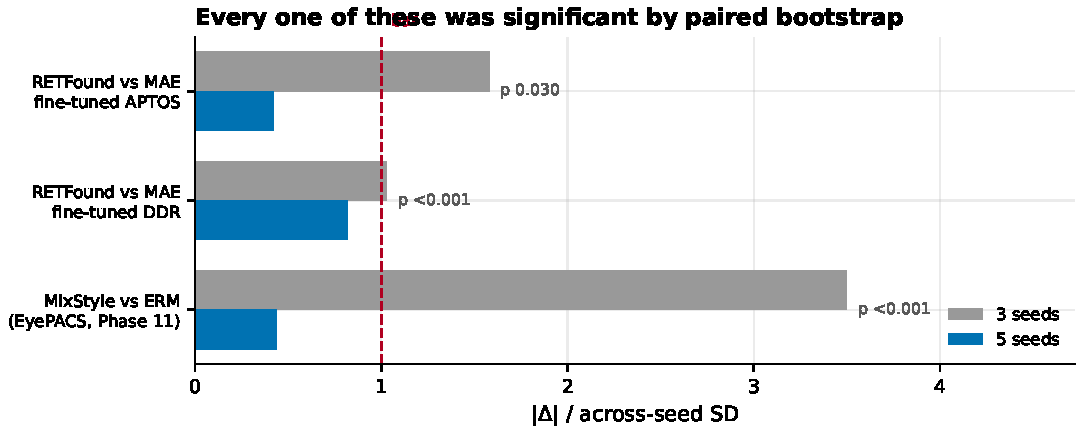
\includegraphics[width=\columnwidth]{../outputs/figures/fig2_seed_collapse.pdf}
\caption{Three effects that were significant under a paired bootstrap at three
seeds and fell below the seed-variance bar at five.}
\label{fig:seeds}
\end{figure}

\subsection{No DG objective beats ERM}
Table~\ref{tab:dg} gives the comparison. On the EyePACS target
(35{,}108 test images, five methods, two samplers, three seeds) no method
clears both bars. The domain-balanced sampler removes the
obvious objection: it drives degenerate batches from 62\% to 0\% for GroupDRO
and 61\% to 0\% for IRM, and the ranking does not change. The result replicates
on DDR. IRMv1 diverged to NaN on all DDR seeds under its published annealing
schedule and again under a schedule matched to the split's iteration count;
we report this as instability rather than as a method comparison.

\subsection{What does move cross-domain performance}
\label{sec:resolution}
Fig.~\ref{fig:ranking} ranks the interventions tested. The largest effect is a
change of input configuration from 224\,px at batch 32 to 512\,px at batch 16:
$+0.0967$ QWK on EyePACS ($4.8\times$ SD) with severe misgrades down 22--48\%
across targets. A modern architecture at comparable cost (ConvNeXt-Tiny) is
second at $+0.0554$ ($4.1\times$). Every domain-generalization objective, and
domain-specific pretraining under partial fine-tuning, are within seed noise.

\textbf{Decomposing the configuration.} The two configurations differ in
resolution \emph{and} batch size, because 512\,px at batch 32 does not fit the
8\,GB budget these experiments were run under. We therefore ran the missing
224\,px/batch-16 cell, which splits the change into a batch contrast
(224/32 to 224/16, resolution held) and a resolution contrast
(224/16 to 512/16, batch held). Table~\ref{tab:configuration} gives both, on
the two held-out domains that have a 512\,px arm and over the three seeds
common to all three configurations.

The two domains do not answer alike. On EyePACS the batch contrast is
$+0.0103$ QWK, smaller than its own across-seed SD and not even consistent in
sign across seeds, while the resolution contrast is $+0.0865$ --- nearly
nine-tenths of the combined $+0.0967$. On IDRiD the split is closer to even:
$+0.0459$ from batch and $+0.0421$ from resolution.

\textbf{The batch-controlled resolution effect is established on EyePACS}
(Holm-corrected $p=0.030$ on the per-seed effects). IDRiD shows a positive
effect on all three seeds but remains underpowered at the seed level
($p=0.088$), and the batch contrast reaches significance on neither domain.
We therefore claim isolated resolution only where it is established, quote the
batch-controlled estimate rather than the confounded one, and treat IDRiD's
split as a point estimate rather than a result.

Three limits bound this. Three seeds is a very small basis for seed-level
inference: the exact sign-flip permutation test cannot return a two-sided $p$
below $0.2500$ at $n=3$, so it cannot reach significance here for any effect
size, and it is reported as a sensitivity check rather than as evidence. The
decomposition exists only for EyePACS and IDRiD, the two held-out domains with
a 512\,px arm; no isolated resolution effect is claimed for DDR or APTOS, whose
comparisons remain the combined configuration. And the in-domain 512\,px runs
have no 224\,px/batch-16 counterpart, so in-domain resolution is still a
configuration effect and is reported as one.

\begin{table}[t]
\centering
\caption{Decomposition of the 224\,px / 512\,px comparison. Every 512\,px run in this study used batch 16, because 512\,px at batch 32 does not fit in 8\,GB of VRAM, so resolution and batch size moved together and the effect reported previously was a configuration effect. Adding the missing 224\,px/batch-16 cell separates them: the batch contrast holds resolution fixed, the resolution contrast holds batch fixed, and the combined contrast is the original comparison. Intervals are from the crossed seed $\times$ case bootstrap; $p_{\text{Holm}}$ is corrected within each contrast across held-out domains, not across contrasts, because the combined contrast is the sum of the other two and is not an independent hypothesis. Positive favours the second configuration.}
\label{tab:configuration}
\begin{tabular}{llrrrrrr}
\toprule
Contrast & Held-out & seeds & $\Delta$ QWK & 95\% CI & seed SD & sign & $p_{\text{Holm}}$ \\
\midrule
Batch (224/32 $\to$ 224/16) & EyePACS & 3 & $+0.0103$ & $[-0.0140, +0.0299]$ & 0.0230 & 2/3 & 0.521 \\
 & IDRiD & 3 & $+0.0459$ & $[-0.0027, +0.0974]$ & 0.0424 & 3/3 & 0.403 \\
\addlinespace
Resolution (224/16 $\to$ 512/16) & EyePACS & 3 & $+0.0865$ & $[+0.0686, +0.1036]$ & 0.0184 & 3/3 & 0.030 \\
 & IDRiD & 3 & $+0.0421$ & $[+0.0052, +0.0807]$ & 0.0231 & 3/3 & 0.088 \\
\addlinespace
Combined (224/32 $\to$ 512/16) & EyePACS & 3 & $+0.0967$ & $[+0.0802, +0.1190]$ & 0.0201 & 3/3 & 0.028 \\
 & IDRiD & 3 & $+0.0880$ & $[+0.0476, +0.1376]$ & 0.0260 & 3/3 & 0.028 \\
\bottomrule
\end{tabular}
\end{table}


\begin{figure}[t]
\centering
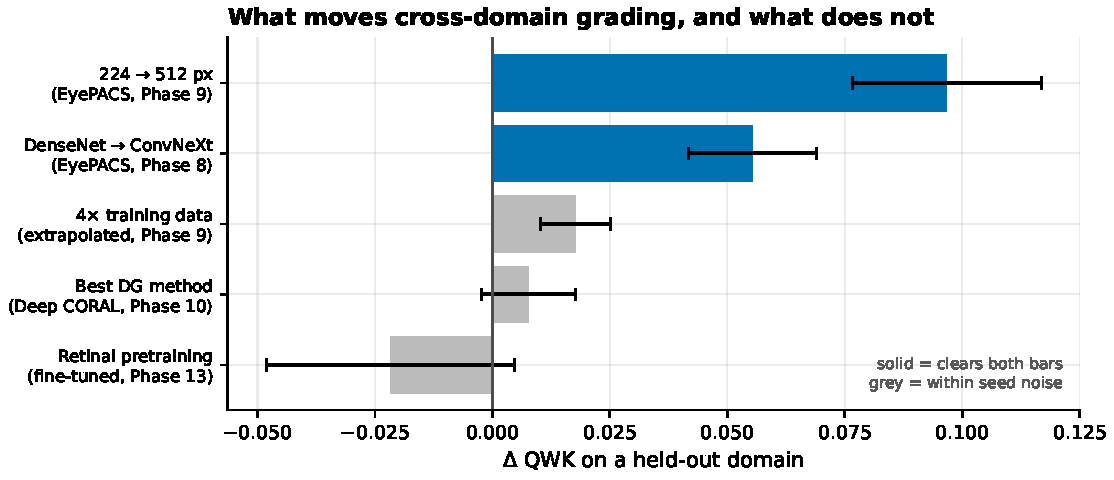
\includegraphics[width=\columnwidth]{../outputs/figures/fig3_intervention_ranking.pdf}
\caption{Best observed effect on a held-out domain for each intervention, with
the across-seed standard deviation it must clear.}
\label{fig:ranking}
\end{figure}

\subsection{The cost of cross-domain deployment}
Table~\ref{tab:deployment} and Fig.~\ref{fig:landscape} give the
comparison. Against in-domain models evaluated on identical test images,
deployment to an unseen domain costs $0.138$ QWK on DDR and $0.291$ on EyePACS, with severe
misgrades rising 107\% and 155\% respectively. A subsampling study attributes
6\% of the EyePACS gap to training-set size and 94\% to domain shift.

\begin{table*}[t]
\centering
\caption{RETFound against the ImageNet MAE checkpoint it was initialised from, under two evaluation protocols. Architecture, parameter count, objective, splits, augmentation and schedule are identical; the pretraining corpus is the only variable. $\Delta$ is ImageNet-MAE minus RETFound, so a positive value favours the general-purpose initialisation. $\sigma$ is the standard deviation of the paired per-seed differences. Bold marks effects clearing both criteria of Section~\ref{sec:bars}; every other entry is within seed noise. The frozen protocol reports an advantage on two of three held-out domains and the fine-tuned protocol on none.}
\label{tab:foundation}
\begin{tabular}{lrrrrrr}
\toprule
& \multicolumn{3}{c}{Frozen (linear probe)} & \multicolumn{3}{c}{Fine-tuned (last 4 of 24 blocks)} \\
\cmidrule(lr){2-4}\cmidrule(lr){5-7}
Held-out domain & seeds & $\Delta$ QWK & $|\Delta|/\sigma$ & seeds & $\Delta$ QWK & $|\Delta|/\sigma$ \\
\midrule
DDR & 10 & $\mathbf{+0.0626}$ & 2.46 & 5 & $+0.0217$ & 0.82 \\
APTOS 2019 & 10 & $\mathbf{+0.1134}$ & 2.07 & 5 & $+0.0073$ & 0.42 \\
IDRiD & 10 & $-0.0429$ & 1.25 & 5 & $\mathbf{-0.0423}$ & 1.13 \\
\bottomrule
\end{tabular}
\end{table*}

\begin{table}[t]
\centering
\caption{Domain-generalization objectives against ERM under a naturally shuffled sampler, on the two held-out domains tested. No method clears both criteria on either domain. IRMv1 diverged to NaN on every DDR seed, under its published annealing schedule and again under one matched to the split's iteration count, and is recorded as diverged rather than scored.}
\label{tab:dg}
\begin{tabular}{llrrrr}
\toprule
Held-out & Method & QWK & $\Delta$ vs ERM & $|\Delta|/\sigma$ & seeds \\
\midrule
EYEPACS & deep coral & 0.4225 & $+0.0077$ & 0.77 & 3 \\
EYEPACS & mixstyle & 0.4091 & $-0.0056$ & 0.23 & 3 \\
EYEPACS & groupdro & 0.4142 & $-0.0005$ & 0.30 & 3 \\
EYEPACS & irm & 0.3379 & $\mathbf{-0.0768}$ & 4.73 & 3 \\
DDR & deep coral & 0.7338 & $-0.0046$ & 0.62 & 3 \\
DDR & mixstyle & 0.7444 & $+0.0061$ & 0.44 & 3 \\
DDR & groupdro & 0.7333 & $-0.0051$ & 0.71 & 3 \\
\bottomrule
\end{tabular}
\end{table}


\begin{table}[t]
\centering
\caption{The cost of cross-domain deployment. An in-domain model and a leave-one-domain-out model are evaluated on the same matched test images and differenced seed-to-seed over three seeds, so the reported spread is the run-to-run variation of the difference itself rather than of either model alone. $\Delta$ is LODO minus in-domain, so a negative value is the cost of never having seen the domain. Bold marks the two entries clearing both criteria of Section~\ref{sec:bars}. IDRiD's positive value is within seed noise and must not be read as cross-domain training helping.}
\label{tab:deployment}
\begin{tabular}{lrrrr}
\toprule
Domain & In-domain QWK & LODO QWK & $\Delta$ & Paired 95\% CI \\
\midrule
DDR & 0.8702 $\pm$ 0.0086 & 0.7327 $\pm$ 0.0038 & $\mathbf{-0.1376}$ & $[-0.1760, -0.0954]$ \\
APTOS 2019 & 0.9085 $\pm$ 0.0097 & 0.8625 $\pm$ 0.0103 & $-0.0460$ & $[-0.1002, +0.0035]$ \\
IDRiD & 0.5846 $\pm$ 0.0191 & 0.6803 $\pm$ 0.0504 & $+0.0957$ & $[-0.1630, +0.3661]$ \\
EyePACS & 0.7063 $\pm$ 0.0139 & 0.4153 $\pm$ 0.0082 & $\mathbf{-0.2910}$ & $[-0.3305, -0.2375]$ \\
\bottomrule
\end{tabular}
\end{table}


\begin{figure}[t]
\centering
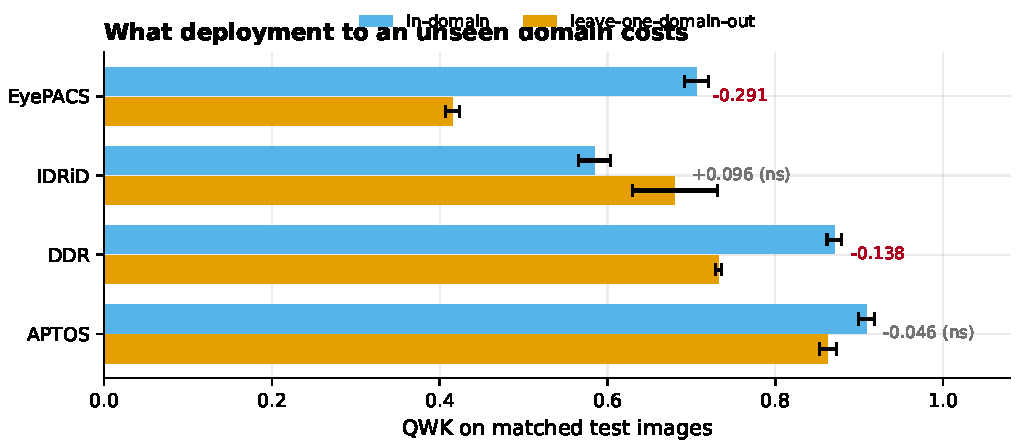
\includegraphics[width=\columnwidth]{../outputs/figures/fig5_lodo_landscape.pdf}
\caption{In-domain and leave-one-domain-out models on the same matched test
images, three seeds each, paired seed-to-seed. Annotations give the paired
difference; \emph{ns} marks the two domains where it does not clear both
criteria of Section~\ref{sec:bars}.}
\label{fig:landscape}
\end{figure}

% ------------------------------------------------------------- discussion
\section{Discussion}
The practical reading is narrow and, we think, useful. We do not claim that
retinal pretraining is harmful. We claim that a linear probe and a fine-tune
rank these two models differently on the same data, that the frozen result is
the larger and more eye-catching of the two, and that it is the one a cheap
benchmark would report.

This matters because probe-based evaluation is common precisely where compute is
scarce, which is also where practitioners are most likely to adopt a foundation
model on the strength of a published benchmark. Our results suggest that such a
benchmark answers a different question from the deployment one.

The broader pattern across this study is that interventions which improve
in-domain fit do not reliably improve cross-domain transfer, and that the
intervention which helped most --- input resolution --- is the one the
domain-generalization literature does not study.

% ------------------------------------------------------------ limitations
\section{Limitations}
\label{sec:limits}
\begin{itemize}
\item \textbf{Partial fine-tuning.} The last 4 of 24 blocks were unfrozen. Full
      fine-tuning is affordable on the hardware used and remains untested.
\item \textbf{IDRiD is the smallest target} (507 test images). Its frozen
      per-seed effect survives correction while its crossed interval, which
      also resamples cases, spans zero; we report both and claim neither.
      Case-level uncertainty dominates at this test-set size.
\item \textbf{Pretraining provenance rests on the publication.} DDR, APTOS
      and IDRiD are not in RETFound's published colour-fundus corpus, whose
      composition is enumerated. The released checkpoint carries no manifest,
      so this is what the primary source establishes, not a verified audit.
\item \textbf{One modality, one task, four datasets}, with documented label
      quality problems in at least two.
\item \textbf{No clinical validation.} No reader study and no deployment data.
\item \textbf{Nulls are not equivalences.} Two of the three partially fine-tuned
      targets are non-significant, not demonstrated equal.
\end{itemize}

% ------------------------------------------------------------- conclusion
\section{Conclusion}
Frozen probing and partial fine-tuning yield materially different point
estimates of the relative advantage of the two initialisations, although the
direct protocol interaction is not statistically established at the current
seed budget. In our matched comparison the cheap protocol favours the
general-purpose initialisation on two of three held-out domains, while under
partial fine-tuning no domain shows a difference surviving correction. We note
that this is partial fine-tuning of the last 4 of 24 blocks, not full
fine-tuning, and the two should not be equated. Reported alongside a leave-one-domain-out
study in which no domain-generalization objective beat ERM and input resolution
beat all of them, the results suggest that measurement protocol deserves as much
scrutiny in this area as method design.

\section*{Data Availability and Ethics}
This work is a secondary analysis of de-identified, publicly available fundus
photography datasets. No human participants were recruited and no new patient
data were collected or accessed by the authors. Each dataset was obtained from
its canonical public source and used in accordance with the terms under which
it is distributed. \todo{per-dataset licence table, and confirm institutional
requirements for secondary analysis of public data --- do not assert that
approval was not required until this is confirmed}

\section*{Reproducibility}
The experiment registry is an append-only log of \num{302} entries covering
\num{288} unique configurations, of which \num{283} completed and \num{5}
diverged; a further \num{9} log entries were superseded by a later run of the
same configuration. Only the completed configurations contribute results, and
these five counts are not interchangeable. Every
table and figure in this paper is emitted by a script from that registry, and a
consistency audit verifies the derived tables against it. Runs that diverged are
recorded as such rather than omitted.

\bibliographystyle{IEEEtran}
\bibliography{refs}

\end{document}
